\documentclass{asaproc}

\usepackage{amsmath}
\usepackage{float}
%\usepackage{times}
%If you have times installed on your system, please
%uncomment the line above

\usepackage{natbib}
\usepackage[export]{adjustbox}

\newtheorem{defn}{Definition}
%For figures and tables to stretch across two columns
%use \begin{figure*} \end{figure*} and
%\begin{table*}\end{table*}
% please place figures & tables as close as possible
% to text references
\usepackage{graphicx}

\newcommand{\prodi}{\prod_{i=1}^n}
\newcommand{\sumi}{\sum_{i=1}^n}
\newcommand\tab[1][1cm]{\hspace*{#1}}
\newcommand{\Pois}{\text{Pois}}
\newcommand{\Gam}{\text{Gamma}}
\newcommand{\be}{\begin{equation}}
\newcommand{\ee}{\end{equation}}
 \title{Red Hawk Sightings in California}

%input all authors' names

\author{Mary Silva\\
AMS 207 - Take Home Exam 1}

%input affiliations

%{USDA Forest Service Forest Products Laboratory}

\begin{document}

\maketitle

%\begin{figure}[h]
%    \includegraphics[width=0.5\textwidth]{Rplot05.pdf}
%    \caption{Airport locations}
%    \label{fig:loc}
%\end{figure}




\begin{abstract}
The North American Breeding survey provides information about the abundance of different species of birds in North America. We look to examine the counts of Red Hawk sightings in California using a Bayesian Hierarchical model.
\begin{keywords}
Hierarchical model, rejection sampling, Poisson-Gamma model, North American Breeding Survey.
\end{keywords}
\end{abstract}

\begin{table}[ht]
\centering
\caption{A portion of the data from North American Breeding Survery for the years 1968 - 1977 showing the counts of Red-tailed Hawks in California and the Route Counts for each year.}
\label{BirdDat}
\begin{tabular}{rrrr}\\\\
  \hline
 & years & Route Count & Red-tailed Hawk \\ 
  \hline
1 & 1968 &  26 &  73 \\ 
  2 & 1969 &  31 &  81 \\ 
  3 & 1970 &  59 & 157 \\ 
  4 & 1971 &  59 & 131 \\ 
  5 & 1972 & 128 & 307 \\ 
  6 & 1973 & 151 & 284 \\ 
  7 & 1974 & 145 & 364 \\ 
  8 & 1975 & 150 & 381 \\ 
  9 & 1976 & 144 & 405 \\ 
  10 & 1977 & 144 & 367 \\ 
   \hline
\end{tabular}

\end{table}



\section{Introduction}
The data is obtained from the North American Breeding Survey for Red Hawks in California (Table \ref{BirdDat}). The full data set contains the years 1977 through 2017. The variables of interest are the bird route counts and the counts of Red Hawk sightings.

Initial exploratory analysis shows an increasing trend of Red Hawk sightings over time (Figure \ref{scatter_Eda}) as well as an increasing trend in bird flight route counts (Figure \ref{Routes}). We see that the density for red hawk sightings in California \ref{HistDensOriginal} is multimodal and skewed, which should be taken into consideration when building a model.

\begin{figure}
    \centering
    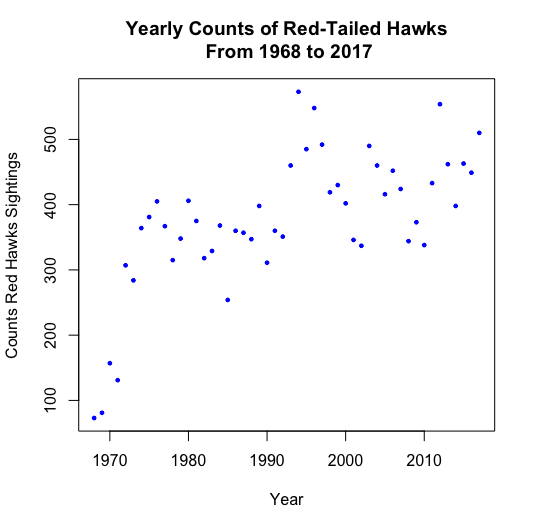
\includegraphics[scale=0.4]{Scatter_EDA.png}
    \caption{Scatter plot of the counts of Red Hawk Sightings by year in California}
    \label{scatter_Eda}
\end{figure}

\begin{figure}
    \centering
    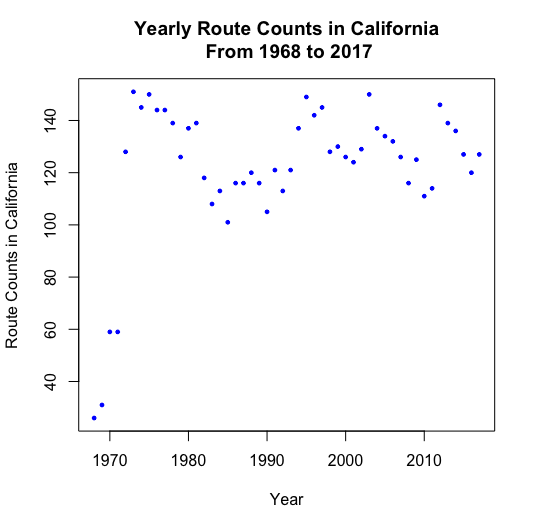
\includegraphics[scale=0.4]{Routes.png}
    \caption{Scatter plot of the route counts for California over time}
    \label{Routes}
\end{figure}
\begin{figure}
    \centering
    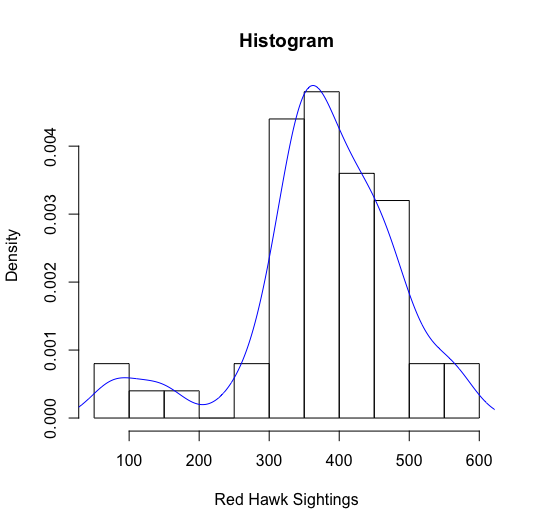
\includegraphics[scale=0.35]{Hist_Dens.png}
    \caption{A histogram plot of the Red Hawk sightings in California with a density overlay}
    \label{HistDensOriginal}
\end{figure}

\section{Model Methodology}
Given that we are dealing with count data, it is reasonable to consider the red hawk sightings $(y_i)$ to be distributed from a Beta-Binomial model, or as Poisson-Gamma model. 
\subsection{Model 1: Methodology}
For this data, we'll first attempt the following hierarchical structure:
\begin{align*}
    y_i &\sim \Pois(\mu_i)\\
    \mu_i &\sim \Gam(\alpha, \beta)\\
    \beta &\sim \Gam(a, b) 
\end{align*}
where $\mu_i = \lambda_i/c_i$ and $c_i$ represents the route count for the i-th year. Furthermore, we will assume $\alpha_b, \beta_b$ and $\alpha$ are fixed. Later, we will assign a prior to alpha as well.

The joint posterior distribution for the above mentioned model then becomes
\begin{align*}
    p(\mu, \beta | y) &\propto \prodi \left[ f(y|\mu_i) p(\mu_i|\alpha,\beta) \right]p(\beta)\\
    &\propto \prodi \mu_i^{y_i + \alpha -1} exp\left\{-(\beta + 1) \sumi \mu_i \right\}
    \\
    &\tab \times\frac{b^a}{\Gamma(a)} \beta^{a-1} \exp\left\{-b\beta\right\}
\end{align*}

The full conditionals (up to proportionality) under this model specification are as follows
\begin{align*}
    \mu_i|\cdot &\sim \Gam\Big(y_i + \alpha, \beta + 1\Big)\\
    \beta|\cdot &\sim \Gam\left(\alpha n + a, b + \sumi \mu_i\right)
\end{align*}

Since the full conditionals (under this model specification) are known distributions, we can use R to implement Gibbs sampling algorithms to simulate from the joint posterior of all parameters.

We use 2000 MCMC iterations and discard  a burn-in of 1000 iterations so sample from the full conditionals. Since this is a Gibbs algorithm, our hyper parameters can be specified as vague. In this case we set $\alpha = 10, a = 1$, and $b = 1$. We summarize our posterior samples in (Table \ref{summary_m1}). A brief analysis of the traceplots and histograms shows that our Gibbs sampler is mixing and converging properly (Appendix Figure \ref{m1_TraceHists}). We also can verify that there are no issues with autocorrelation (Figure \ref{acf1}) which further prove that the Gibbs sampler is working.

\begin{table}[h!]
\centering
\label{summary_m1}
\caption{Summary of posterior means of select posterior samples of $\mu$ and $\beta$. Keep in mind that $\mu_i = \lambda_i/c_i$}
\begin{tabular}{rrrrr}
  \hline
 & Mean & Sd & 2.5\% & 97.5\% \\ 
  \hline
$\mu_1$ & 80.36 & 8.78 & 63.57 & 98.03 \\ 
  $\mu_{10}$ & 366.88 & 19.44 & 329.15 & 406.17 \\ 
  $\mu_{30}$ & 488.38 & 21.52 & 446.05 & 533.37 \\ 
  $\mu_{49}$ & 447.20 & 21.28 & 408.08 & 488.53 \\ 
  $\beta$ & 0.03 & 0.00 & 0.02 & 0.03 \\ 
   \hline
\end{tabular}
\end{table}

\begin{figure}[h!]
    \centering
        \caption{Distribution of the observed $y_i$ and the distributions of some of the posterior replicates ($y_i^{rep}$) from model 1.}
    \label{m1_replicates}
    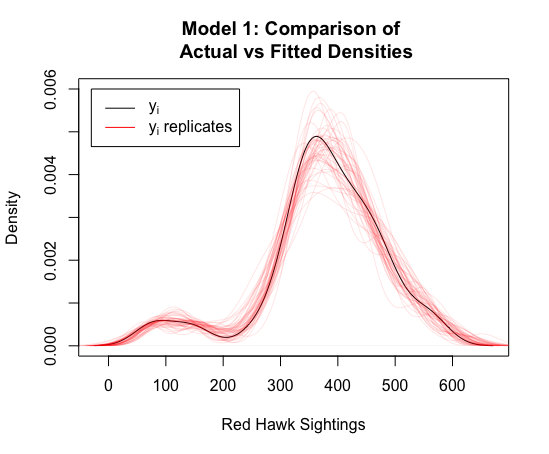
\includegraphics[scale = 0.3]{m1_fittedDens.png}
\end{figure}
\begin{figure}[h!]
    \centering
        \caption{Posterior  predictive  distribution, $T(y)=mean(y)$. We compare the mean of the observed to the means of the $y_i^{\textit{rep}}$}
    \label{m1_meanHist}
    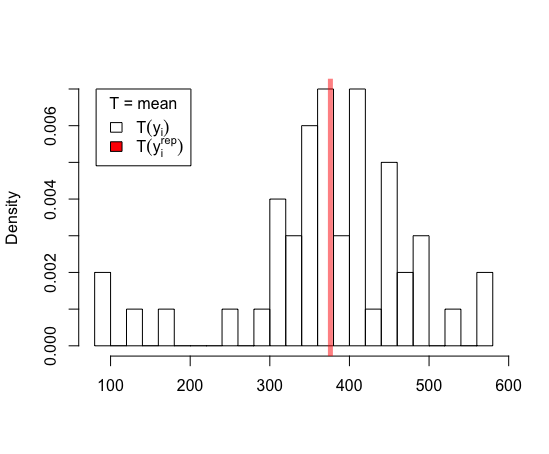
\includegraphics[scale = 0.3]{m1_meanHist.png}
\end{figure}

\subsection{Model 1: Model Assessment}
Next, we present predictive model checks and provide an assessment of the model fit to the observed records. Under the model 1 specifications, we simulate 200 posterior replicates of $y_i$ (Figure \ref{m1_replicates}). We see that under this model specification, the posterior density fits very well (maybe too well). 



We may also compare the means of the posterior predictive destribution to the mean of the observed results (Figure \ref{m1_meanHist}). Based on the model 1 specifications, we can conclude this model accurately fits the data.


\section{Model 2: Methodology}
Next, we propose a hierarchical model similar to model 1, but also adds a prior on $\alpha$ as follows
\begin{align*}
    y_i &\sim \Pois(\mu_i)\\
    \mu_i &\sim \Gam(\alpha, \beta)\\
    \beta &\sim \Gam(a, b) \\
    \alpha &\sim \Gam(c,d)
\end{align*}

Where, here, the fixed parameters are $a,b,c$ and $d$. The joint posterior distribution for model 2 then becomes

\begin{align*}
    p(\mu, \beta, \alpha|y) & \propto \prodi \left[f(y_i|\mu_i) p(\mu_i|\alpha,\beta) \right] p(\alpha) p(\beta)\\
    &\propto \left(\frac{\beta^{\alpha n}}{\Gamma(\alpha)^n} \right) \prodi \left( \mu_i ^{y_i + \alpha -1}\right) \\
    &\tab\times\exp\left\{
    -\sumi \mu_i \left(1 + \beta\right)\right\}\\
    &\tab \times \frac{b^a}{\Gamma(a)} \alpha^{a-1} \exp\left\{-b\alpha\right\}\\
    &\tab \times\frac{d^c}{\Gamma(c)} \beta^{c-1} \exp\left\{-d\beta \right\}
\end{align*}

From this, we can obtain the full conditionals (up to proportionality).
\begin{align*}
    p(\mu_i|\cdot) &\propto \mu_i^{y_i + \alpha -1} \exp \Big\{-\mu_i(\beta+1) \Big\}\\
    p(\beta|\cdot) & \propto \beta^{\alpha n + c -1} \exp\left\{-\beta\left(d +\sumi \mu_i\right)\right\}\\
    p(\alpha|\cdot) &\propto \left(\prodi \mu_i^\alpha\right)\frac{\beta^{\alpha n}}{\Gamma(\alpha)^n}  \alpha^{a-1} \exp\left\{-b\alpha \right\}
\end{align*}

We recognize that the full conditionals for $\mu_i$ and $\beta$ are known distributions, thus

\begin{align*}
    \mu_i|\cdot &\sim \Gam(y_i + \alpha, \beta +1)\\
    \beta|\cdot &\sim \Gam(\alpha n + c, d + \sumi \mu_i)
\end{align*}

The full conditional for $\alpha$, however, is not a known standard distribution. Thus, we must apply either a Metropolis-within-Gibbs step or rejection sampling method to sample the $\alpha$'s. Using both methods, almost identical results were obtained, but for this paper only a Sampling Importance Resampling (SIR) method is used to jointly sample $(\alpha, \beta)$. 

The computational procedure is as follows
\begin{itemize}
    \item Draw from the joint posterior $p(\alpha, \beta) \propto p(\alpha) p(\beta)$
    \item Given $\alpha,\beta$, draw $\mu_i$ from the corresponding Gamma distribution
\end{itemize}

A contour plot of $\alpha$ and $\beta$ on the log scale for model 2, together with simulated draws from the rejection algorithm, are shown in Figure \ref{contour}. A summary of the posterior samples can be seen in Table \ref{m2_table}. We can note that these values are similar to model 1.

\begin{figure}[h!]
    \centering
    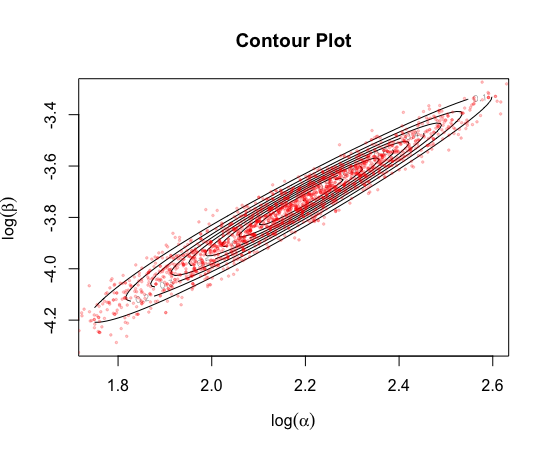
\includegraphics[scale = 0.4]{Contour.png}
    \caption{Contour plot with 2000 samples of $\alpha$ and $\beta$ on the log scale.}
    \label{contour}
\end{figure}


\begin{table}[ht]
\centering
\label{m2_table}
\caption{Cap}
\begin{tabular}{rrrrr}
  \hline
 & Mean & SD & 2.5\% & 97.5\% \\ 
  \hline
$\alpha$ & 8.79 & 1.72 & 5.75 & 12.39 \\ 
  $\beta$ & 0.02 & 0.00 & 0.02 & 0.03 \\ 
  $\mu_1$ & 79.81 & 8.92 & 63.40 & 98.54 \\ 
  $\mu_2$ & 87.86 & 9.48 & 69.65 & 108.25 \\ 
  $\mu_3$ & 161.88 & 12.74 & 138.64 & 187.76 \\ 
  $\mu_4$ & 136.32 & 11.80 & 113.68 & 159.85 \\ 
 $\mu_5$ & 309.41 & 17.67 & 275.85 & 345.99 \\ 
   \hline
\end{tabular}
\end{table}

Again, to check for mixing and convergence we examine the sampling traces for the parameters (Appendix Figures \ref{m2alphabetamu1} - \ref{m2mu2}). By examining the traceplots of $\mu_1$ for both models, we see that the parameter converges almost identically to the same mean (It's not the same image, I triple checked!). The autocorrelation plots also show no problems (\Figure \ref{acf2}).

\clearpage
\subsection{Model 2: Model Assessment}
We repeat the assesment steps as we did with model 1. The comparison of the actual Red Hawk sightings to the posterior predictive replicates, $y_i^{rep}$, (Figure \ref{m2replicates}) are expected to look identical for both models and we can see that this is true. The reason for this is that with model 1, we set $\alpha = 10$ in order to reflect the distributional assumptions allowing us to obtain the good estimates for $\mu_i = \lambda_i/c_i$. This choice of $\alpha$ in model 1 happens to be very close to the posterior mean for $\alpha$ in model 2 which explains the similar fitted values.



\begin{figure}[h!]
    \centering
    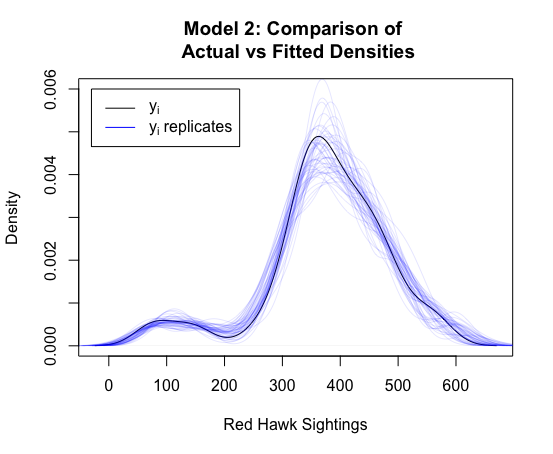
\includegraphics[scale = 0.4]{m2_replicates.png}
    \caption{Distribution of the observed $y_i$ and the distributions of some of the posterior replicates ($y_i^{rep}$) for Model 2.}
    \label{m2replicates}
\end{figure}

\section{Conclusion}
As we expected, both model 1 and model 2 yield similar results. We can use a model comparison method to verify this. 

\begin{defn}[Gelfand \& Ghosh]
Let $\pmb{y}$ denote the observed data. Let $\mu_l = E(z_l|\pmb{y})$ and $\sigma^2_l = Var(z_l|\pmb{y})$. Then let $G = \sum_l (\mu_l - y_l)^2$, and $P = \sum_l \sigma^2_l$. The Gelfand and Ghosh criterion is defined as $D = G + P$, where $D$ seeks to reward goodness of fit penalizing complexity. So the smaller the D, the better the model.
\label{GG}
\end{defn}

The Gelfand \& Ghosh criterion for model 1 is 2449.3 and for model 2 is 2678.6. Since the Gelfand and Ghosh Criterion for model 1 is smaller this, by definition, indicates that model 1 fits the data better. The smaller value for model 1 is expected since model 2 is more complex and GG penalizes complexity. Of course, there are other methods to compare model fit, such as Deviance Information Criterion (DIC), and Bayes Factor, but those methods will be applied to future assignments once they are covered in the course. 




\clearpage
\begin{figure*}[th!]
    \centering
    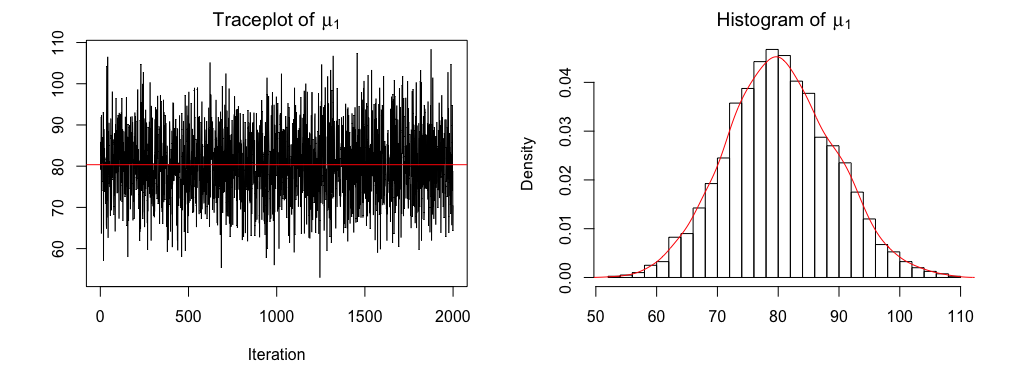
\includegraphics[scale = 0.4]{m1_mu1.png}\\
    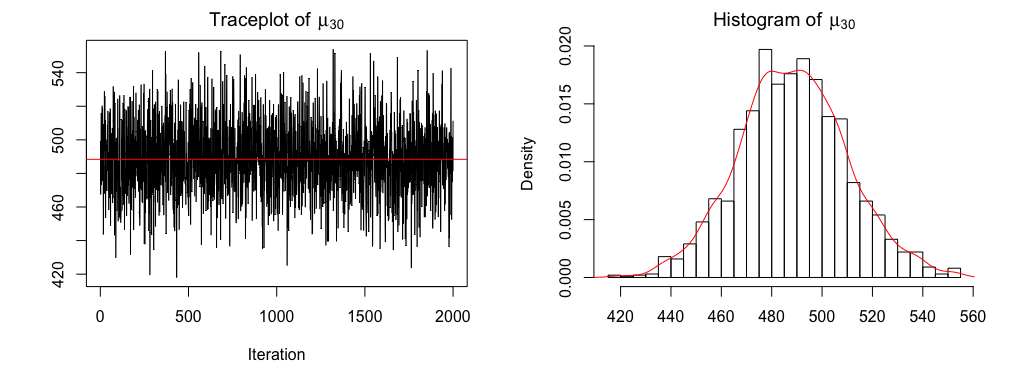
\includegraphics[scale = 0.4]{m1_mu30.png}\\
    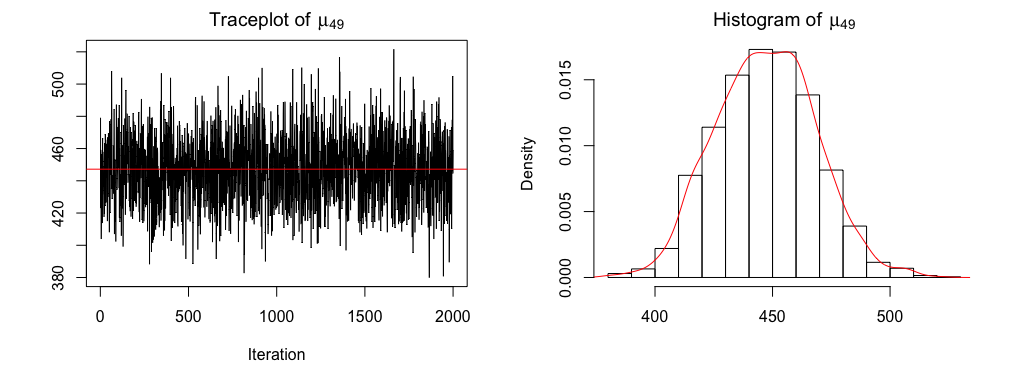
\includegraphics[scale = 0.4]{m1_mu49.png}\\
    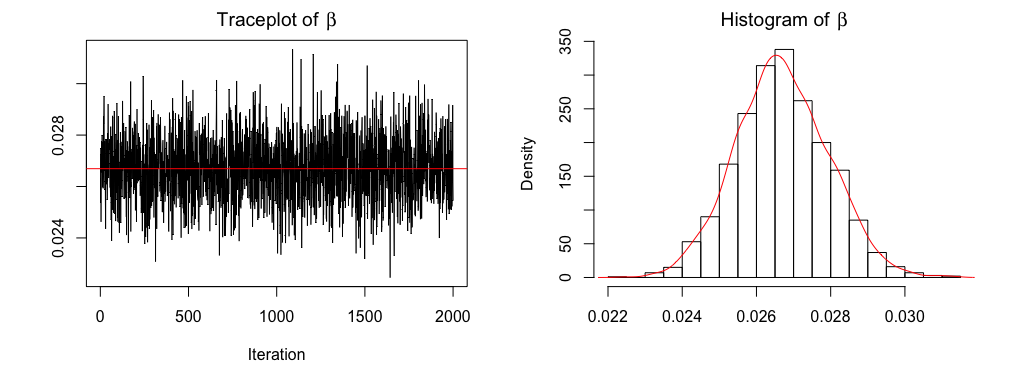
\includegraphics[scale = 0.4]{m1_betas.png}
    \caption{Traceplots for $\mu_{1},\mu_{30},\mu_{49}$, and $\beta$.}
    \label{m1_TraceHists}
\end{figure*}

\begin{figure*}
    \centering
    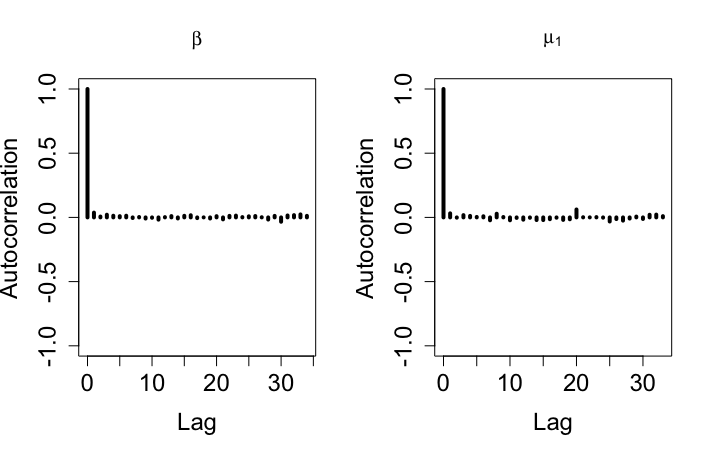
\includegraphics[scale = 0.6]{acf_m1.png}
    \caption{Autocorrelation for model 1 parameters $\beta, \mu_1$}
    \label{acf1}
\end{figure*}


\begin{figure*}
    \centering
    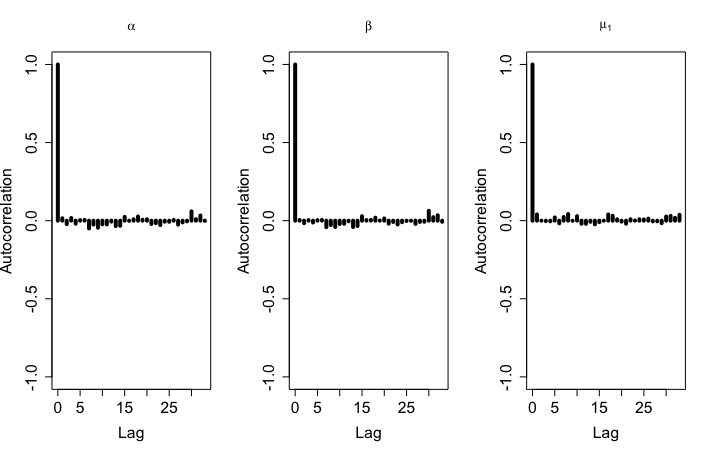
\includegraphics[scale = 0.7]{acf_m2.png}
    \caption{Autocorrelation for model 2 parameters $\alpha, \beta, \mu_1$}
    \label{acf2}
\end{figure*}

\begin{figure*}
    \centering
    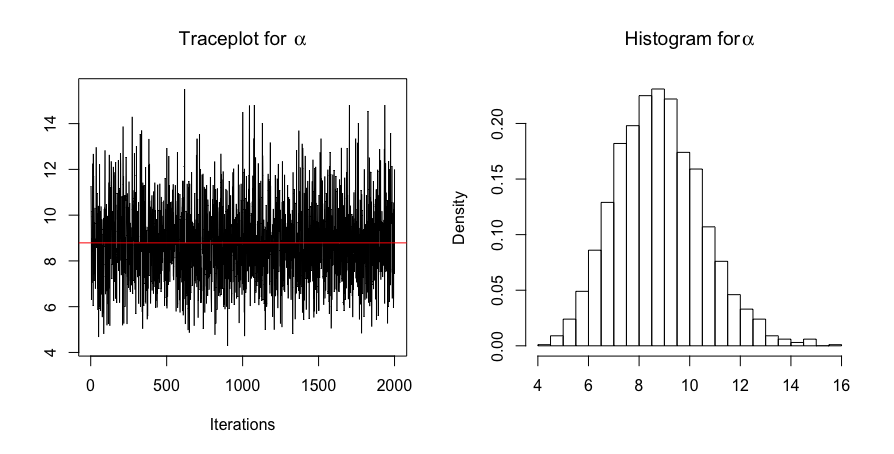
\includegraphics[scale = 0.5]{m2_alpha.png}\\
    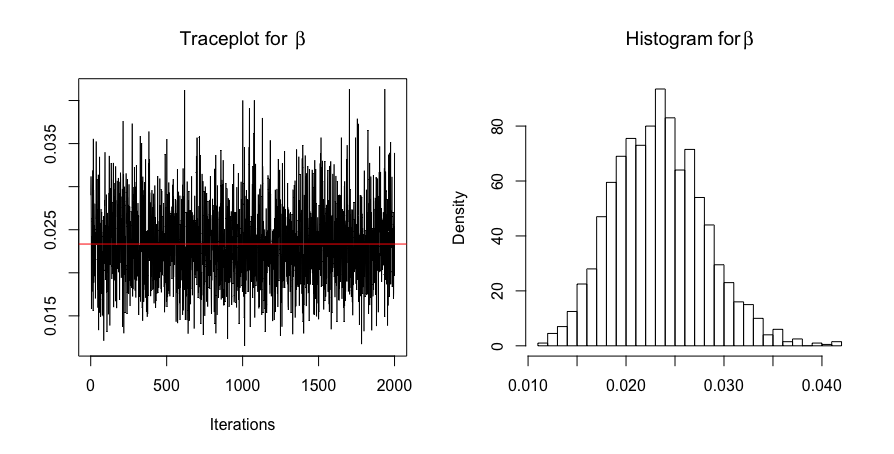
\includegraphics[scale = 0.5]{m2_beta.png}\\
    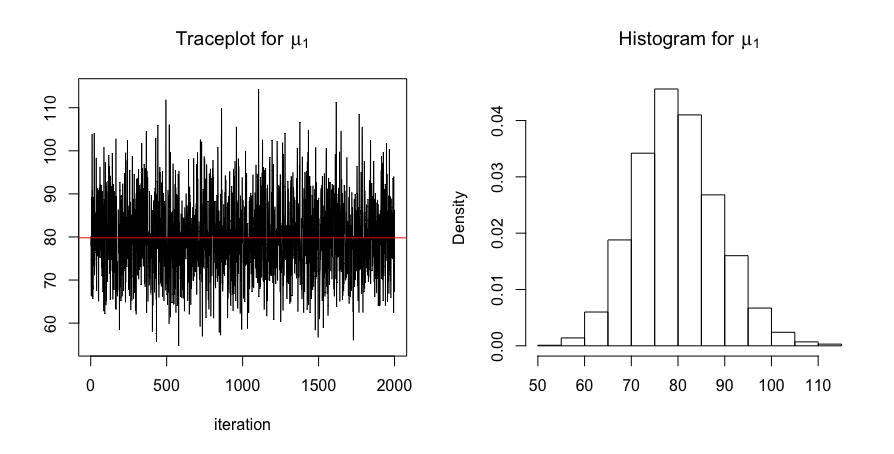
\includegraphics[scale = 0.5]{m2_mu1.png}
    \caption{Traceplots and histograms for posterior samples of $\alpha, \beta$ and $\mu_1$ corresponding to model 2.}
    \label{m2alphabetamu1}
\end{figure*}

\begin{figure*}
    \centering
    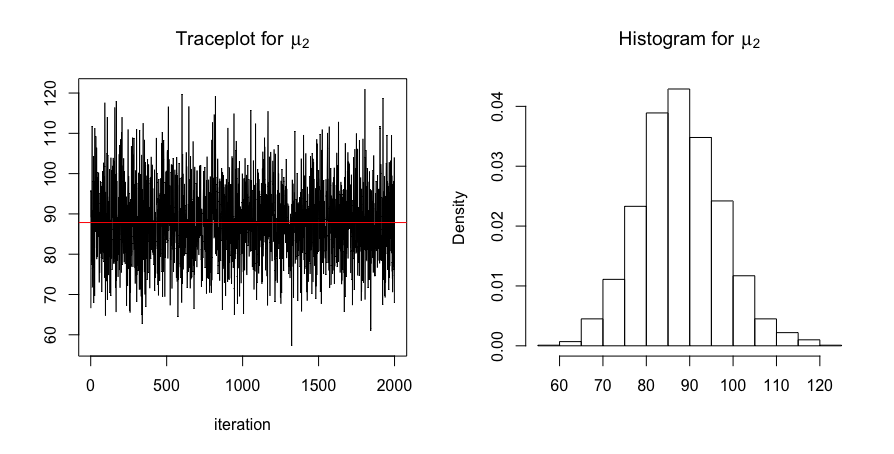
\includegraphics[scale = 0.5]{m2_mu2.png}
    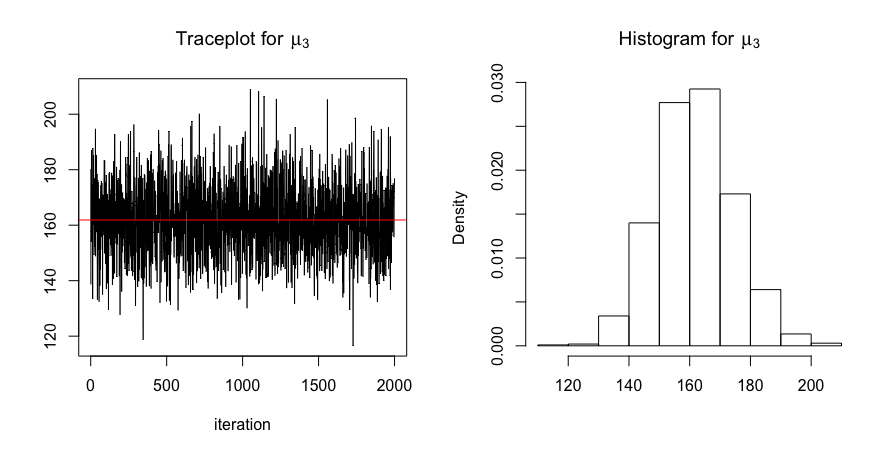
\includegraphics[scale = 0.5]{m2_mu3.png}
    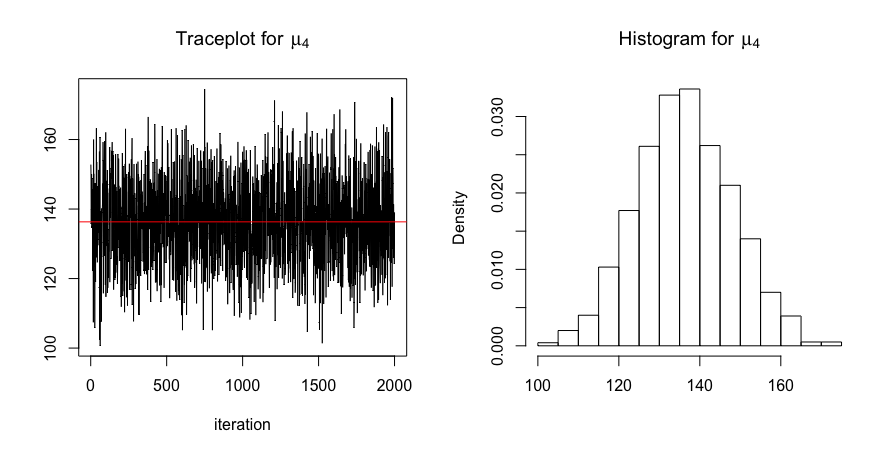
\includegraphics[scale = 0.5]{m2_mu4.png}
    \caption{Traceplots and histograms for posterior samples of $\mu_{i}$ for $i=2,...,4$. Clearly, convergence is achieved.}
    \label{m2mu2}
\end{figure*}

To estimate the probability of observing more than 450 red hawks in california in a year with a route count of 120, I sampled 2500 iterations from the route counts from gamma distribution and kept the results where the rate was greater than 120, and set all others equal to 0. Then I used the vector of route counts where this statement was true to simulate 2500 y posterior predictive replicates. From this, I calculated the percentage of values where the result was greater than 450. This percentage came out to be around 22.4\%. This compares well to the 26\% in the original data.
\end{document}